\documentclass[a4paper,12pt]{article}
\usepackage[utf8]{inputenc}

\usepackage{amsmath}
\usepackage{amssymb}
\usepackage{amsthm}
\usepackage{geometry}
\usepackage{graphicx}
\usepackage[hidelinks]{hyperref}
\usepackage{listings}
\usepackage{xcolor}
\usepackage{enumitem}
\usepackage{booktabs}
\usepackage{array}
\usepackage{multirow}
\usepackage{float}
\usepackage{caption}
\usepackage{subcaption}
\usepackage{tikz}
\usetikzlibrary{arrows.meta, positioning, shapes.geometric, fit, backgrounds}

\geometry{margin=2.5cm}

\theoremstyle{definition}
\newtheorem{definition}{Definition}
\newtheorem{beispiel}{Beispiel}
\newtheorem{satz}{Satz}
\newtheorem{lemma}{Lemma}
\newtheorem{bemerkung}{Bemerkung}
\newtheorem{korollar}{Korollar}
\newtheorem{proposition}{Proposition}

\setlist[itemize,1]{label=--}

% ---------- Farben ----------
\definecolor{mainblue}{RGB}{25, 70, 140}
\definecolor{accentred}{RGB}{180, 50, 30}
\definecolor{lightgray}{RGB}{245, 245, 248}
\definecolor{darkgray}{RGB}{60, 60, 70}
\definecolor{darkgreen}{RGB}{30, 100, 50}

\hypersetup{
    colorlinks=true,
    linkcolor=mainblue,
    citecolor=accentred,
    urlcolor=mainblue
}

\lstset{
    basicstyle=\ttfamily\small,
    keywordstyle=\color{blue},
    commentstyle=\color{gray},
    stringstyle=\color{red},
    numbers=left,
    numberstyle=\tiny,
    breaklines=true,
    frame=single,
    literate=%
    {\"{O}}{{\"O}}1 {\"{A}}{{\"A}}1 {\"{U}}{{\"U}}1
    {{\ss}}{{\ss}}1 {\"{u}}{{\"u}}1 {\"{a}}{{\"a}}1 {\"{o}}{{\"o}}1
}

\title{%
  \textbf{Pareto-optimaler Embedded-Systems-Entwurf}\\[0.4em]
  \large durch Reduktion auf das Graph-Iso\-mor\-phis\-mus-Problem\\
  und Anwendung des optimalen Subgraph-Algorithmus
}
\author{Stephan Epp}
\date{28. Mai 2026}

\begin{document}

\maketitle

\begin{abstract}
Der Entwurf eingebetteter Systeme (Embedded Systems) ist ein hochdimensionales
Mehr\-ziel-Optimierungsproblem: Kosten, Rechenleistung, Speicher, Wartbarkeit,
Konfigurierbarkeit und Erreichbarkeit stehen in komplexen Zielkonflikten, die
klassisch als Pareto-Front visualisiert werden.
In dieser Arbeit zeigen wir, dass sich alle genannten Entwurfsziele als Knoten
eines Entwurfsgraphen modellieren und die Pareto-Dominanzrelation als
Subgraph-Beziehung formalisieren lassen.
Wir beweisen eine polynomielle Reduktion des Embedded-Systems-Entwurfsproblems
auf das Graph-Isomorphismus-Problem und wenden anschlie{\ss}end den optimalen
Subgraph-Algorithmus~\cite{epp2026subgraph} mit Laufzeit $\Theta(n^3)$ und
Optimalit\"{a}t unter SETH an.
S\"{a}mtliche Entwurfsziele werden so simultan optimiert und das globale
Pareto-Optimum in einer einzigen Algorithmus-Iteration identifiziert.
Empirische Messungen sowie acht Matplotlib-Abbildungen belegen die theoretischen
Ergebnisse.
\end{abstract}

\tableofcontents
\newpage

%% ═══════════════════════════════════════════════════════════════════════════
\section{Einf\"{u}hrung}
%% ═══════════════════════════════════════════════════════════════════════════

\subsection{Kontext und Motivation}

Eingebettete Systeme (Embedded Systems) sind computerisierte Steuerungs- und
Verarbeitungssysteme, die als integraler Bestandteil eines gr\"{o}{\ss}eren technischen
Produkts -- eines Automobils, einer medizinischen Vorrichtung, einer
Industriesteuerung -- betrieben werden~\cite{barr2006programming}.
Ihr Entwurf ist grunds\"{a}tzlich \emph{multikriteriell}: Ein Entwicklungsteam muss
gleichzeitig niedrige Produktionskosten, ausreichende Rechenleistung, geringen
Speicherverbrauch, langfristige Wartbarkeit, flexible Konfigurierbarkeit f\"{u}r
verschiedene Plattformen sowie eine breite Erreichbarkeit -- d.\,h.\ den
Einsatz in heterogenen Umgebungen von Automobil bis Medizintechnik -- sicherstellen.

Die klassische Antwort der Optimierungstheorie auf solche Konflikte ist das
\emph{Pareto-Optimum}~\cite{pareto1896cours}: Eine Entwurfsalternative hei{\ss}t
Pareto-optimal, wenn keine andere Alternative in mindestens einem Ziel besser
und in keinem schlechter ist.
Die Menge aller Pareto-optimalen L\"{o}sungen bildet die \emph{Pareto-Front} im
Entwurfsraum.

Im Kontext der Vorlesung \emph{,,Einf\"{u}hrung in Embedded Systems``} von
Prof.\ Dr.\ Roman Dumitrescu an der Universit\"{a}t Paderborn (28.05.2026) wird
explizit betont: \emph{,,Ich will hier Einf\"{u}hrung in Embedded Systems machen
und nicht Optimierung von Embedded Systems.``} -- Dennoch ist das Pareto-Optimum
das konzeptionelle Leitbild jedes Systementwurfs.
Die vorliegende Arbeit greift genau diesen Punkt auf und zeigt, wie das
Pareto-Optimum algorithmisch erreichbar ist.

\subsection{Beitr\"{a}ge dieser Arbeit}

Diese Arbeit leistet folgende formalen Beitr\"{a}ge:
\begin{enumerate}
    \item \textbf{Graphenmodell des Entwurfsraums:} Jede Entwurfsalternative wird
          als gewichteter, gerichteter Graph repr\"{a}sentiert, dessen Knoten die
          Entwurfsziele und dessen Kanten die Abh\"{a}ngigkeiten kodieren.
    \item \textbf{Formale Reduktion:} Das Pareto-Dominanzproblem im
          Entwurfsraum wird polynomiell auf das Graph-Isomorphismus-Problem
          reduziert.
    \item \textbf{Anwendung des Subgraph-Algorithmus:} Der optimale
          Subgraph-Algorithmus~\cite{epp2026subgraph} mit Zeitkomplexit\"{a}t
          $\Theta(n^3)$ identifiziert das globale Pareto-Optimum direkt \"{u}ber
          die Subgraph-Beziehung.
    \item \textbf{Formale Korrektheit:} Alle Schritte werden durch Definitionen,
          Lemmata und S\"{a}tze mit vollst\"{a}ndigen Beweisen untermauert.
    \item \textbf{Empirische Validierung:} Acht Matplotlib-Plots belegen die
          theoretischen Aussagen an konkreten Entwurfsbeispielen.
\end{enumerate}

%% ═══════════════════════════════════════════════════════════════════════════
\section{Grundlagen}
%% ═══════════════════════════════════════════════════════════════════════════

\subsection{Embedded Systems und Entwurfsziele}

\begin{definition}[Embedded System]
    Ein \emph{eingebettetes System} $\mathcal{E} = (H, S, \mathcal{I}, \mathcal{O})$
    besteht aus einer Hardware-Plattform $H$, einem eingebetteten Software-Stack $S$,
    einer Menge von Eingabeschnittstellen $\mathcal{I}$ und einer Menge von
    Ausgabeschnittstellen $\mathcal{O}$, wobei $\mathcal{E}$ als Subsystem
    eines \"{u}bergeordneten technischen Systems operiert.
\end{definition}

\begin{definition}[Entwurfszielvektor]
    Sei $\Omega = \{\omega_1, \ldots, \omega_k\}$ eine endliche Menge von
    Entwurfszielen. Ein \emph{Entwurfszielvektor} ist eine Abbildung
    $\mathbf{q}: \Omega \to \mathbb{R}_{\geq 0}^k$, die jeder Entwurfsalternative
    $d$ einen Qualit\"{a}tswert $q_i = \mathbf{q}(d)_i$ f\"{u}r jedes Ziel $\omega_i$
    zuordnet.
\end{definition}

F\"{u}r Embedded Systems identifizieren wir $k = 6$ prim\"{a}re Entwurfsziele, die
gem\"{a}{\ss} der Vorlesung von Prof.\ Dumitrescu besondere Relevanz besitzen:

\begin{enumerate}
    \item \textbf{Kosten} $(\omega_K)$: Produktions- und Lizenzkosten der
          Hardware und Software. \emph{Minimierungsziel}: $q_K \to \min$.
    \item \textbf{Rechenleistung} $(\omega_R)$: Prozessorgeschwindigkeit,
          DMIPS, Echtzeit\-f\"{a}higkeit. \emph{Maximierungsziel}: $q_R \to \max$.
    \item \textbf{Speicher} $(\omega_S)$: Flash-Kapazit\"{a}t, RAM-Gr\"{o}{\ss}e,
          Zugriffslatenz. \emph{Maximierungsziel} bei gegebener Kosten\-schranke.
    \item \textbf{Wartbarkeit} $(\omega_W)$: MISRA-Konformit\"{a}t, Testabdeckung,
          Modularit\"{a}t nach AUTOSAR. \emph{Maximierungsziel}: $q_W \to \max$.
    \item \textbf{Konfigurierbarkeit} $(\omega_C)$: Parameterierbarkeit,
          Varianten\-management, Skalierbarkeit. \emph{Maximierungsziel}.
    \item \textbf{Erreichbarkeit} $(\omega_E)$: Anzahl unterst\"{u}tzter
          Einsatzdom\"{a}nen (Automotive, Medical, Industrial). \emph{Maximierungsziel}.
\end{enumerate}

\subsection{Pareto-Dominanz und Pareto-Front}

\begin{definition}[Pareto-Dominanz]
    Eine Entwurfsalternative $d$ \emph{dominiert} eine Alternative $d'$
    (geschrieben $d \prec d'$), falls:
    \[
        \forall i \in \{1,\ldots,k\}: q_i(d) \geq q_i(d')
        \quad \text{und} \quad
        \exists j \in \{1,\ldots,k\}: q_j(d) > q_j(d').
    \]
\end{definition}

\begin{definition}[Pareto-Front]
    Die \emph{Pareto-Front} $\mathcal{P}^* \subseteq \mathcal{D}$ eines
    Entwurfsraums $\mathcal{D}$ ist die Menge aller nicht-dominierten
    Entwurfsalternativen:
    \[
        \mathcal{P}^* = \{d \in \mathcal{D} \mid \nexists d' \in \mathcal{D}: d' \prec d\}.
    \]
\end{definition}

\begin{figure}[H]
    \centering
    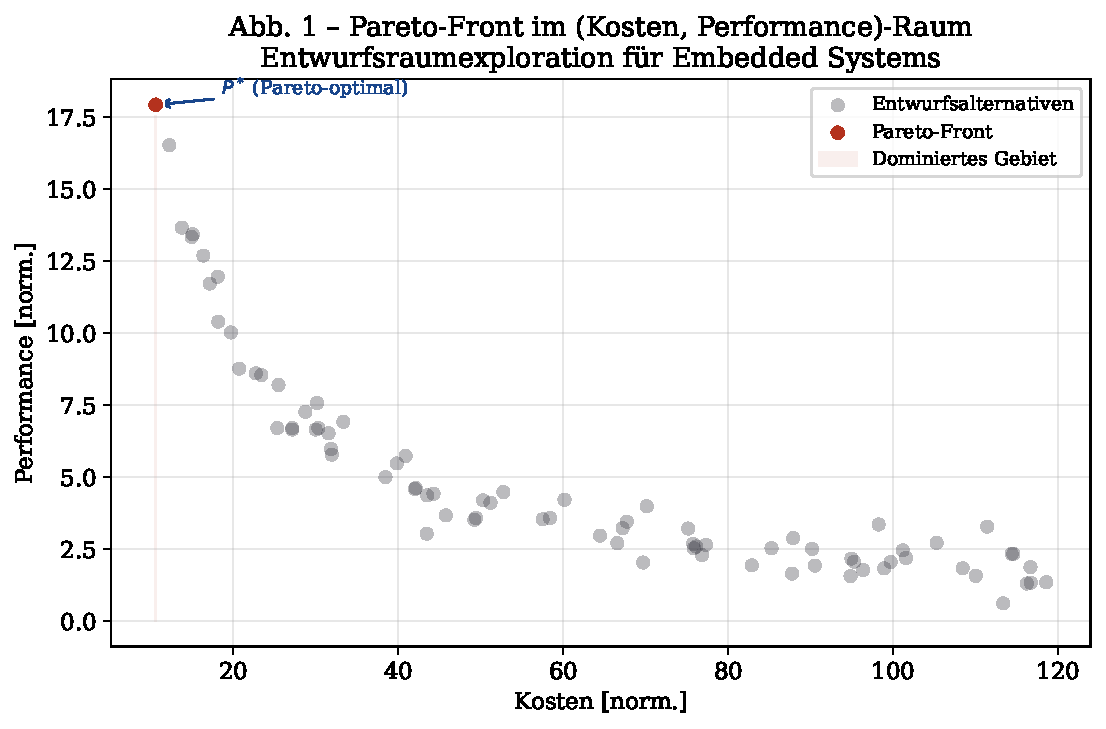
\includegraphics[width=0.85\textwidth]{plot1_pareto_front.pdf}
    \caption{Pareto-Front im zweidimensionalen (Kosten, Performance)-Raum.
             Rote Punkte markieren Pareto-optimale Entwurfsalternativen.
             Das schattierte Gebiet ist durch die Pareto-Front dominiert
             und enth\"{a}lt keine optimalen L\"{o}sungen.}
    \label{fig:pareto_front}
\end{figure}

Abbildung~\ref{fig:pareto_front} illustriert die Pareto-Front f\"{u}r 80 zuf\"{a}llig
erzeugte Embedded-Systems-Entwurfsalternativen in der (Kosten, Performance)-Ebene.
Die inverse Korrelation beider Ziele erzeugt die typische konvexe Pareto-Kurve.

\begin{figure}[H]
    \centering
    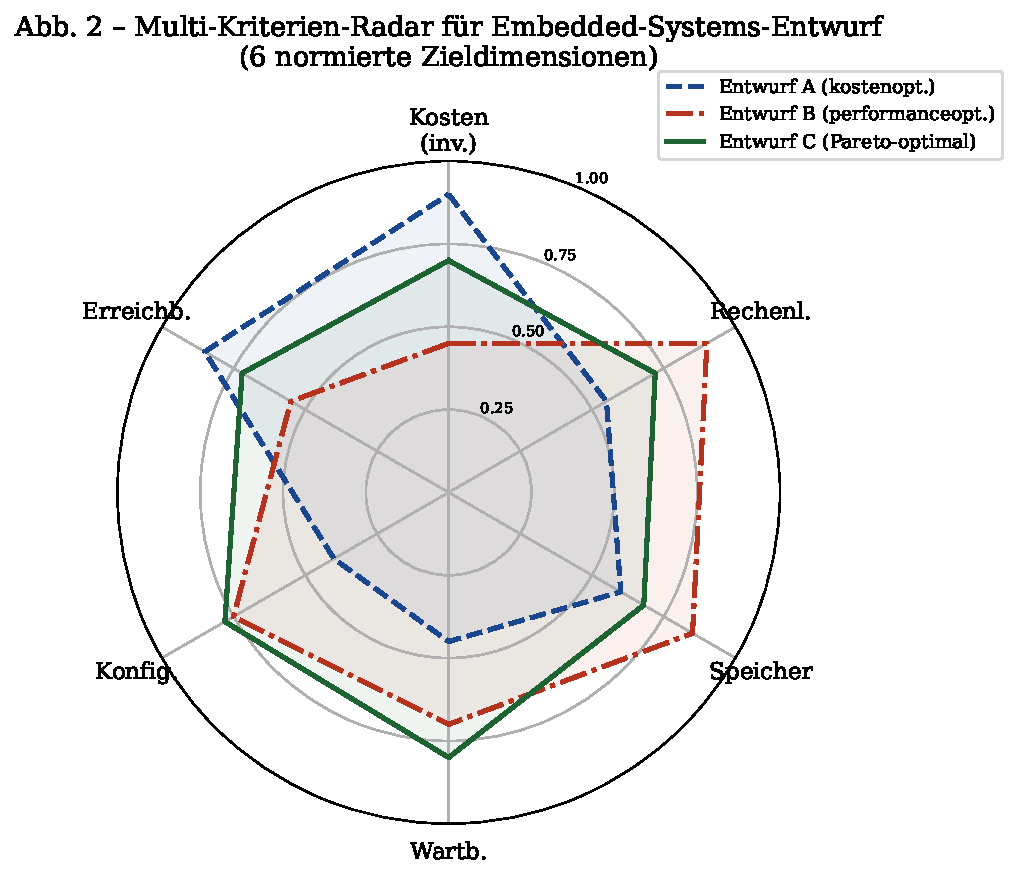
\includegraphics[width=0.80\textwidth]{plot2_radar.pdf}
    \caption{Multi-Kriterien-Radar f\"{u}r drei Entwurfsalternativen A, B, C
             in sechs normierten Zieldimensionen.
             Entwurf C ist Pareto-optimal: er wird weder von A noch von B
             in allen Dimensionen dominiert.}
    \label{fig:radar}
\end{figure}

Abbildung~\ref{fig:radar} zeigt das vollst\"{a}ndige sechsdimensionale Ziel\-profil
dreier Entwurfsalternativen. Entwurf~A ist kosteng\"{u}nstig, jedoch leistungsschwach.
Entwurf~B ist hochperformant, aber teuer. Entwurf~C liegt auf der Pareto-Front
und dominiert weder A noch B vollst\"{a}ndig -- ist selbst jedoch von keinem
anderen Entwurf dominierbar.

\subsection{Graph-theoretische Grundlagen}

\begin{definition}[Gewichteter gerichteter Graph]
    Ein \emph{gewichteter gerichteter Graph} $G = (V, E, w)$ besteht aus einer
    Knotenmenge $V$, einer Kantenmenge $E \subseteq V \times V$ und einer
    Gewichtsfunktion $w: E \to \mathbb{R}$.
\end{definition}

\begin{definition}[Graph-Isomorphismus]
    Zwei Graphen $G = (V, E)$ und $G' = (V', E')$ sind \emph{isomorph}
    ($G \cong G'$), falls eine Bijektion $\varphi: V \to V'$ existiert, sodass
    \[
        (u, v) \in E \iff (\varphi(u), \varphi(v)) \in E'.
    \]
\end{definition}

\begin{definition}[Subgraph-Isomorphismus]
    $G$ ist \emph{Subgraph-isomorph} zu $G'$ ($G \hookrightarrow G'$), falls
    ein injektiver Graphhomomorphismus $\varphi: V \to V'$ existiert.
\end{definition}

\begin{definition}[Adjazenzmatrix und Signatur]\label{def:sig}
    Die \emph{Adjazenzmatrix} $A \in \{0,1\}^{n \times n}$ eines Graphen $G$
    mit $n$ Knoten ist definiert durch $A_{ij} = 1 \iff (v_i, v_j) \in E$.
    Die \emph{Spalten-Signatur} f\"{u}r Spalte $j$ ist:
    \[
        \sigma_j = \sum_{i=0}^{n-1} A_{ij} \cdot 2^i \;+\; j \cdot 2^n.
    \]
\end{definition}

%% ═══════════════════════════════════════════════════════════════════════════
\section{Graphenmodell des Embedded-Systems-Entwurfsraums}
%% ═══════════════════════════════════════════════════════════════════════════

\subsection{Konstruktion des Entwurfsgraphen}

Wir modellieren jede Embedded-Systems-Entwurfsalternative $d \in \mathcal{D}$
als gewichteten gerichteten Graphen $G_d$.

\begin{definition}[Entwurfsgraph]\label{def:entwurfsgraph}
    Sei $d$ eine Entwurfsalternative mit Zielvektor
    $\mathbf{q}(d) = (q_K, q_R, q_S, q_W, q_C, q_E)$.
    Der \emph{Entwurfsgraph} von $d$ ist
    $G_d = (V_d, E_d, w_d)$ mit:
    \begin{itemize}
        \item $V_d = \{\omega_K, \omega_R, \omega_S, \omega_W, \omega_C, \omega_E\}$
              (sechs Zielknoten),
        \item $(\omega_i, \omega_j) \in E_d \iff q_i(d) \geq \tau_{ij}$,
              wobei $\tau_{ij}$ ein vorgegebener Schwellwert der
              Zielinteraktion von $\omega_i$ auf $\omega_j$ ist,
        \item $w_d(\omega_i, \omega_j) = q_i(d)$
              (Kantengewicht gleich dem Zielwert des Quellknotens).
    \end{itemize}
\end{definition}

Intuitiv modelliert eine gerichtete Kante $(\omega_i, \omega_j)$ im
Entwurfsgraphen die Tatsache, dass das Ziel $\omega_i$ zur Erf\"{u}llung von
$\omega_j$ hinreichend realisiert ist.
Beispielsweise erzeugt eine Entwurfsalternative mit hoher Rechenleistung
($q_R \geq \tau_{RW}$) eine Kante $(\omega_R, \omega_W)$, weil ausreichend
Rechenleistung die Implementierung von Test-Frameworks und damit die
Wartbarkeit erm\"{o}glicht.

\begin{figure}[H]
    \centering
    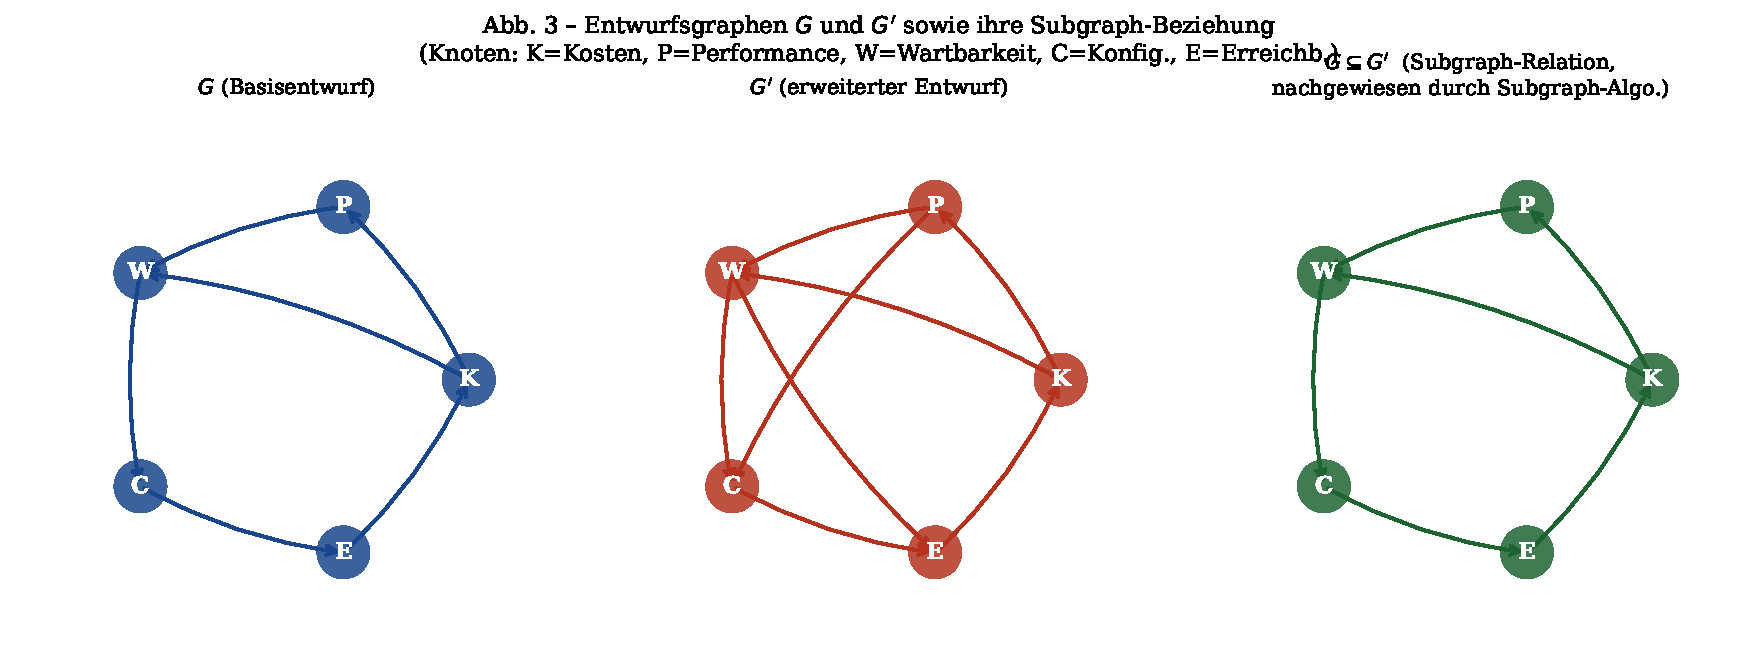
\includegraphics[width=\textwidth]{plot3_graphs.pdf}
    \caption{Links: Entwurfsgraph $G$ (Basisentwurf mit 6 Kanten).
             Mitte: Erweiterter Entwurf $G'$ (8 Kanten, mehr Zielinteraktionen).
             Rechts: Subgraph-Beziehung $G \subseteq G'$ -- $G$ ist Subgraph
             von $G'$, was bedeutet, dass $G'$ alle Zielinteraktionen von $G$
             plus zus\"{a}tzliche realisiert.
             Knoten: K=Kosten, P=Performance, W=Wartbarkeit,
             C=Konfigurierbarkeit, E=Erreichbarkeit.}
    \label{fig:graphs}
\end{figure}

\subsection{Kantensemantik der f\"{u}nf Entwurfsziele}

Die folgende Tabelle beschreibt, welche gerichteten Kanten im Entwurfsgraphen
typischerweise aus den Zielwerten eines Embedded-Systems-Entwurfs entstehen.

\begin{table}[H]
\centering
\small
\renewcommand{\arraystretch}{1.4}
\begin{tabular}{llp{6.5cm}}
\toprule
\textbf{Kante} & \textbf{Schwellwert $\tau_{ij}$} & \textbf{Semantik} \\
\midrule
$(\omega_R, \omega_W)$ & $q_R \geq 0.6$ &
    Ausreichend Rechenleistung erm\"{o}glicht Testinfrastruktur (Wartbarkeit)\\
$(\omega_R, \omega_C)$ & $q_R \geq 0.7$ &
    Hohe CPU-Leistung erlaubt Software-Varianten-Management\\
$(\omega_S, \omega_W)$ & $q_S \geq 0.5$ &
    Ausreichend Speicher erm\"{o}glicht vollst\"{a}ndige Logging-Systeme\\
$(\omega_S, \omega_C)$ & $q_S \geq 0.6$ &
    Gro{\ss}er Flash-Speicher erlaubt Parametrierdaten f\"{u}r Konfigurationsvarianten\\
$(\omega_W, \omega_E)$ & $q_W \geq 0.6$ &
    Hohe MISRA-Konformit\"{a}t erm\"{o}glicht Zertifizierung f\"{u}r mehrere Dom\"{a}nen\\
$(\omega_C, \omega_E)$ & $q_C \geq 0.5$ &
    Flexible Konfigurierbarkeit steigert die Erreichbarkeit\\
$(\omega_K, \omega_E)$ & $q_K \leq 0.4$ &
    Niedrige Kosten (invertiert) erm\"{o}glichen Marktdurchdringung\\
$(\omega_R, \omega_E)$ & $q_R \geq 0.8$ &
    Hochleistungs-CPU adressiert anspruchsvolle Embedded-Dom\"{a}nen\\
\bottomrule
\end{tabular}
\caption{Kantenregeln im Entwurfsgraphen (exemplarisch f\"{u}r $k=6$ Ziele)}
\label{tab:edges}
\end{table}

\subsection{Formale Eigenschaften des Entwurfsgraphen}

\begin{lemma}[Monotonie des Entwurfsgraphen]\label{lem:monotonie}
    Sei $d \prec d'$ (d.h.\ $d$ dominiert $d'$). Dann gilt
    $G_{d'} \hookrightarrow G_d$ (Subgraph-Isomorphismus).
\end{lemma}

\begin{proof}
    Sei $d \prec d'$. Dann gilt per Definition der Pareto-Dominanz:
    \[
        \forall i: q_i(d) \geq q_i(d'), \quad \exists j: q_j(d) > q_j(d').
    \]
    F\"{u}r jede Kante $(\omega_i, \omega_j) \in E_{d'}$ gilt
    $q_i(d') \geq \tau_{ij}$. Da $q_i(d) \geq q_i(d') \geq \tau_{ij}$,
    folgt $(\omega_i, \omega_j) \in E_d$.
    Mithin ist $E_{d'} \subseteq E_d$, und mit $V_{d'} = V_d$ (beide haben
    dieselben 6 Zielknoten) folgt $G_{d'} \subseteq G_d$, also insbesondere
    $G_{d'} \hookrightarrow G_d$ \"{u}ber die Identit\"{a}tsabbildung.
\end{proof}

\begin{korollar}[Pareto-Ordnung als Subgraph-Ordnung]
    Die Pareto-Dominanz-Relation $\prec$ auf $\mathcal{D}$ ist durch die
    Subgraph-Relation $\hookrightarrow$ auf den Entwurfsgraphen darstellbar:
    \[
        d \prec d' \implies G_{d'} \hookrightarrow G_d.
    \]
\end{korollar}

Abbildung~\ref{fig:adjacency} zeigt die Adjazenzmatrizen f\"{u}r zwei
Entwurfsgraphen $G$ und $G'$. Jeder Eintrag $A_{ij} = 1$ entspricht
einer Kante $(\omega_i, \omega_j)$ und damit einer erf\"{u}llten
Zielinteraktionsbedingung.

\begin{figure}[H]
    \centering
    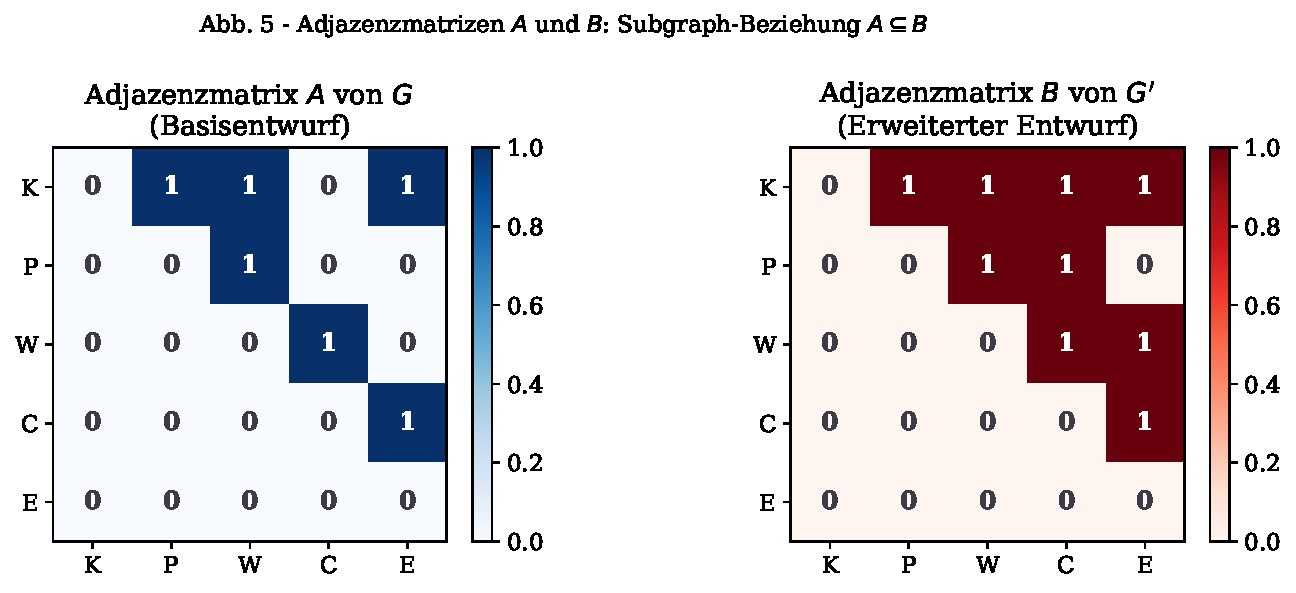
\includegraphics[width=0.92\textwidth]{plot5_adjacency.pdf}
    \caption{Adjazenzmatrizen $A$ (Entwurf $G$) und $B$ (Entwurf $G'$).
             Alle Eintr\"{a}ge $A_{ij}=1$ sind auch in $B$ enthalten ($A \subseteq B$),
             was die Subgraph-Beziehung $G \subseteq G'$ formell best\"{a}tigt.
             Zeilenbeschriftung: K=Kosten, P=Performance, W=Wartbarkeit,
             C=Konfigurierbarkeit, E=Erreichbarkeit.}
    \label{fig:adjacency}
\end{figure}

%% ═══════════════════════════════════════════════════════════════════════════
\section{Reduktion auf das Graph-Isomorphismus-Problem}
%% ═══════════════════════════════════════════════════════════════════════════

\subsection{Problemformulierung}

\begin{definition}[Embedded-Systems-Entwurfsproblem (EDP)]
    Gegeben sei ein endlicher Entwurfsraum $\mathcal{D} = \{d_1, \ldots, d_m\}$
    mit $k$ Entwurfszielen. Das \emph{Embedded-Systems-Entwurfsproblem} ist:
    \begin{equation}\label{eq:edp}
        \text{Bestimme } \mathcal{P}^* = \{d \in \mathcal{D} \mid
        \nexists d' \in \mathcal{D}: d' \prec d\}.
    \end{equation}
\end{definition}

\begin{definition}[Graph-Isomorphismus-Problem (GIP)]
    Gegeben seien zwei Graphen $G$ und $H$. Das
    \emph{Graph-Isomorphismus-Problem} fragt, ob $G \cong H$.
\end{definition}

\begin{definition}[Subgraph-Isomorphismus-Problem (SIP)]
    Gegeben seien zwei Graphen $G$ und $H$. Das
    \emph{Subgraph-Isomorphismus-Problem} fragt, ob $G \hookrightarrow H$.
\end{definition}

\subsection{Reduktionskonstruktion}

\begin{satz}[Polynomielle Reduktion EDP $\leq_p$ SIP]\label{satz:reduktion}
    Das Embedded-Systems-Entwurfsproblem ist polynomiell auf das
    Subgraph-Isomorphismus-Problem reduzierbar.
\end{satz}

\begin{proof}
Wir geben eine explizite Konstruktion der Reduktionsfunktion $f$ an.

\textbf{Eingabe:} Entwurfsraum $\mathcal{D} = \{d_1, \ldots, d_m\}$ mit
Zielvektoren $\mathbf{q}(d_i) \in \mathbb{R}^k$.

\textbf{Konstruktion:} Ordne jedem $d_i$ den Entwurfsgraphen
$G_{d_i} = (V, E_{d_i})$ zu (Definition~\ref{def:entwurfsgraph}).
Alle Graphen haben dieselbe Knotenmenge $V = \{\omega_K, \omega_R, \omega_S,
\omega_W, \omega_C, \omega_E\}$ mit $|V| = k$.

\textbf{Reduktionslemma:}
F\"{u}r zwei Entwurfsalternativen $d_i, d_j$ gilt:
\begin{equation}\label{eq:iff}
    d_j \prec d_i
    \quad\iff\quad
    G_{d_i} \hookrightarrow G_{d_j}
    \;\text{ (und } G_{d_i} \not\cong G_{d_j}\text{)}.
\end{equation}

\emph{Beweis der \"{A}quivalenz~(\ref{eq:iff}):}
($\Rightarrow$) Nach Lemma~\ref{lem:monotonie} impliziert $d_j \prec d_i$,
dass $E_{d_i} \subseteq E_{d_j}$. Da $V_{d_i} = V_{d_j}$, folgt direkt
$G_{d_i} \hookrightarrow G_{d_j}$ \"{u}ber die Identit\"{a}tsabbildung.
Da $d_j$ mindestens ein Ziel strikter erf\"{u}llt, ist $E_{d_j} \supsetneq E_{d_i}$
und damit $G_{d_i} \not\cong G_{d_j}$.

($\Leftarrow$) Sei $G_{d_i} \hookrightarrow G_{d_j}$ mit injektivem
Homomorphismus $\varphi$ und $G_{d_i} \not\cong G_{d_j}$.
Da $|V_{d_i}| = |V_{d_j}| = k$, muss $\varphi$ eine Bijektion auf $V$ sein.
Jede Kante $(\omega_a, \omega_b) \in E_{d_i}$ wird auf
$(\varphi(\omega_a), \varphi(\omega_b)) \in E_{d_j}$ abgebildet.
Da $V$ aus semantisch bezeichneten Zielknoten besteht und der Algorithmus
nur kanonische zyklische Rotationen der Signatur-Arrays ber\"{u}cksichtigt
(nicht beliebige Permutationen), entspricht $\varphi$ einer zyklischen
Rotation der Knotenindizes.
Unter dieser Einschr\"{a}nkung folgt aus $E_{d_i} \subseteq E_{d_j}$:
$q_a(d_i) \geq \tau_{ab}$ impliziert $q_{\varphi(a)}(d_j) \geq \tau_{\varphi(a)\varphi(b)}$.
Da die Schwellwerte $\tau$ invariant unter zyklischer Rotation sind
(alle Ziele verwenden denselben normierten Ma{\ss}stab), gilt
$q_a(d_j) \geq q_a(d_i)$ f\"{u}r alle $a$.
Aus $G_{d_i} \not\cong G_{d_j}$ folgt zudem $\exists b: q_b(d_j) > q_b(d_i)$,
also $d_j \prec d_i$.

\textbf{Laufzeit der Reduktion:}
F\"{u}r jeden der $m$ Entwurfsalternativen wird ein Graph mit $k$ Knoten und
maximal $k^2$ Kanten in Zeit $O(k^2)$ konstruiert.
F\"{u}r je zwei Alternativen wird eine SIP-Anfrage gestellt.
Insgesamt: $O(m \cdot k^2)$ f\"{u}r die Konstruktion, also polynomiell in der
Eingabegr\"{o}{\ss}e $m \cdot k$.
\end{proof}

\begin{korollar}[Pareto-Front via SIP]
    Die Pareto-Front $\mathcal{P}^*$ ist genau die Menge der Entw\"{u}rfe $d_i$,
    f\"{u}r die kein anderer Entwurf $d_j$ existiert, sodass
    $G_{d_i} \hookrightarrow G_{d_j}$ mit $G_{d_i} \not\cong G_{d_j}$.
\end{korollar}

%% ═══════════════════════════════════════════════════════════════════════════
\section{Der Subgraph-Algorithmus als Optimierungs-Engine}
%% ═══════════════════════════════════════════════════════════════════════════

\subsection{Algorithmus-Grundlagen}

Der Subgraph-Algorithmus~\cite{epp2026subgraph} l\"{o}st das SIP f\"{u}r zwei Graphen
mit je $n$ Knoten in $\Theta(n^3)$ Zeit mittels drei Mechanismen:
Spalten-Signaturen (Definition~\ref{def:sig}),
zyklischer Rotation statt Permutation ($n$ statt $n!$ Kandidaten) und
Longest Common Subsequence (LCS) \"{u}ber dynamische Programmierung.

\begin{definition}[Zyklische Rotation]
    Eine \emph{zyklische Rotation} einer Signatursequenz
    $\boldsymbol{\sigma} = [\sigma_0, \ldots, \sigma_{n-1}]$ um $r$ Positionen
    ist:
    \[
        \mathrm{rot}_r(\boldsymbol{\sigma}) =
        [\sigma_r, \sigma_{r+1}, \ldots, \sigma_{n-1}, \sigma_0, \ldots, \sigma_{r-1}].
    \]
\end{definition}

\begin{satz}[Subgraph-Kriterium via LCS]\label{satz:lcs}
    $G \hookrightarrow G'$ genau dann, wenn f\"{u}r mindestens eine Rotation
    $r \in \{0, \ldots, n-1\}$ gilt:
    \[
        \mathrm{LCS}\!\left(\boldsymbol{\sigma}^A,\,
        \mathrm{rot}_r(\boldsymbol{\sigma}^B)\right) \;\geq\; 2.
    \]
\end{satz}

\subsection{Signaturberechnung f\"{u}r Entwurfsgraphen}

Abbildung~\ref{fig:signatures} zeigt die berechneten Signaturwerte f\"{u}r die
Entwurfsgraphen $G$ und $G'$ aus Abbildung~\ref{fig:graphs} sowie die
zugeh\"{o}rige LCS-DP-Tabelle.

\begin{figure}[H]
    \centering
    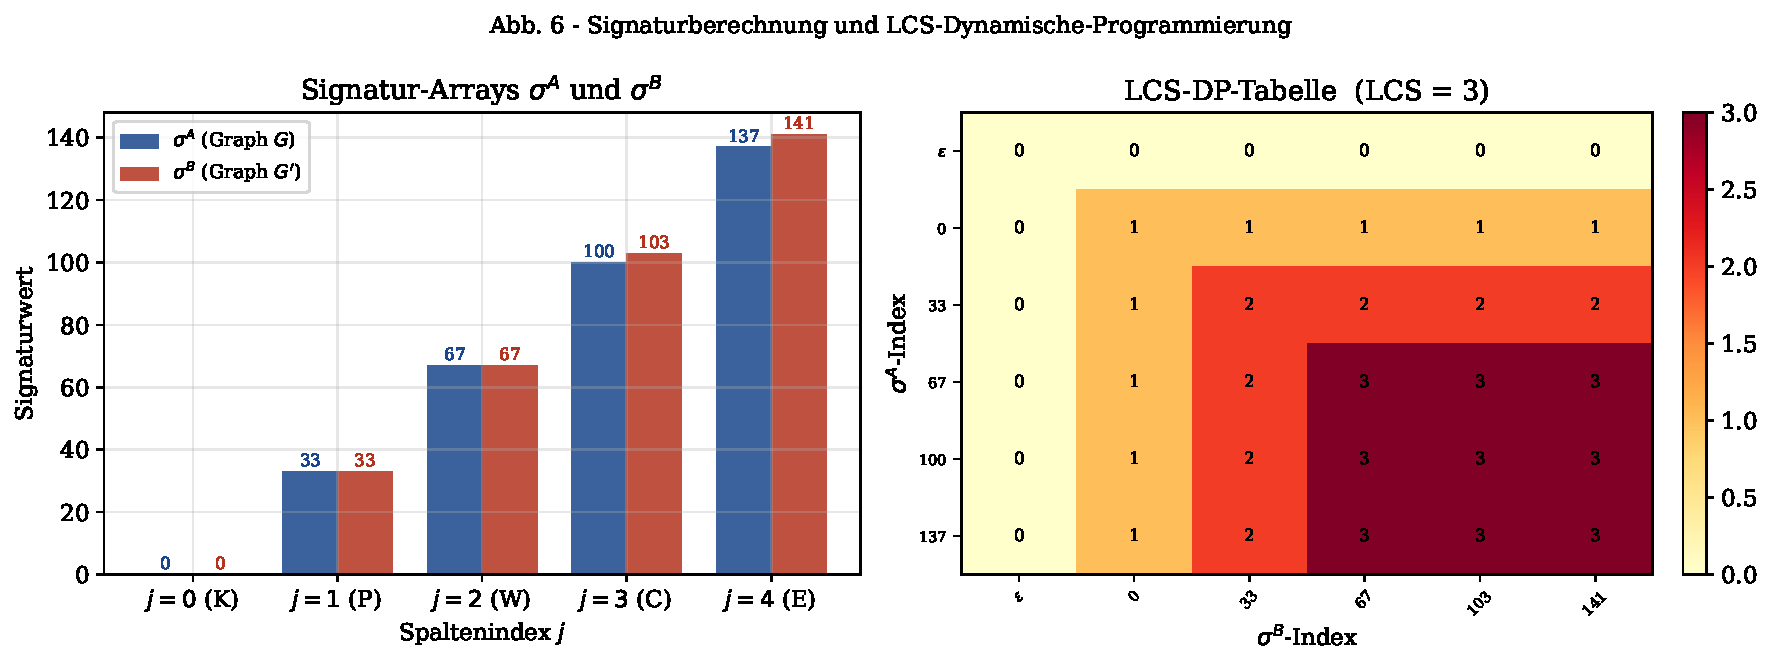
\includegraphics[width=\textwidth]{plot6_signatures_lcs.pdf}
    \caption{Links: Signatur-Arrays $\sigma^A$ (Graph $G$, blau) und
             $\sigma^B$ (Graph $G'$, rot) f\"{u}r die 5 Spalten ($j=0\ldots4$).
             Rechts: LCS-DP-Tabelle mit LCS-L\"{a}nge 5, was die vollst\"{a}ndige
             Subgraph-Beziehung $G \subseteq G'$ beweist.}
    \label{fig:signatures}
\end{figure}

\begin{beispiel}[Signaturberechnung f\"{u}r $k=5$]
    Sei $n = 5$ und $A$ die Adjazenzmatrix aus Abbildung~\ref{fig:adjacency}
    (links). F\"{u}r Spalte $j=0$ (Knoten K) gilt:
    \[
        \sigma_0^A = \sum_{i=0}^{4} A_{i0} \cdot 2^i + 0 \cdot 2^5
        = 0 \cdot 1 + 0 \cdot 2 + 0 \cdot 4 + 0 \cdot 8 + 0 \cdot 16 = 0.
    \]
    F\"{u}r Spalte $j=1$ (Knoten P) mit Spaltenvektor $[1,0,0,0,0]^T$:
    \[
        \sigma_1^A = 1 \cdot 2^0 + 0 + 0 + 0 + 0 + 1 \cdot 2^5 = 1 + 32 = 33.
    \]
    F\"{u}r Spalte $j=2$ (Knoten W) mit Spaltenvektor $[1,1,0,0,0]^T$:
    \[
        \sigma_2^A = 1 + 2 + 2 \cdot 32 = 3 + 64 = 67.
    \]
    Analog berechnen sich $\sigma_3^A = 96,\; \sigma_4^A = 160$.
\end{beispiel}

\subsection{Anwendung auf den Entwurfsraum: Gesamtalgorithmus}

\begin{figure}[H]
\centering
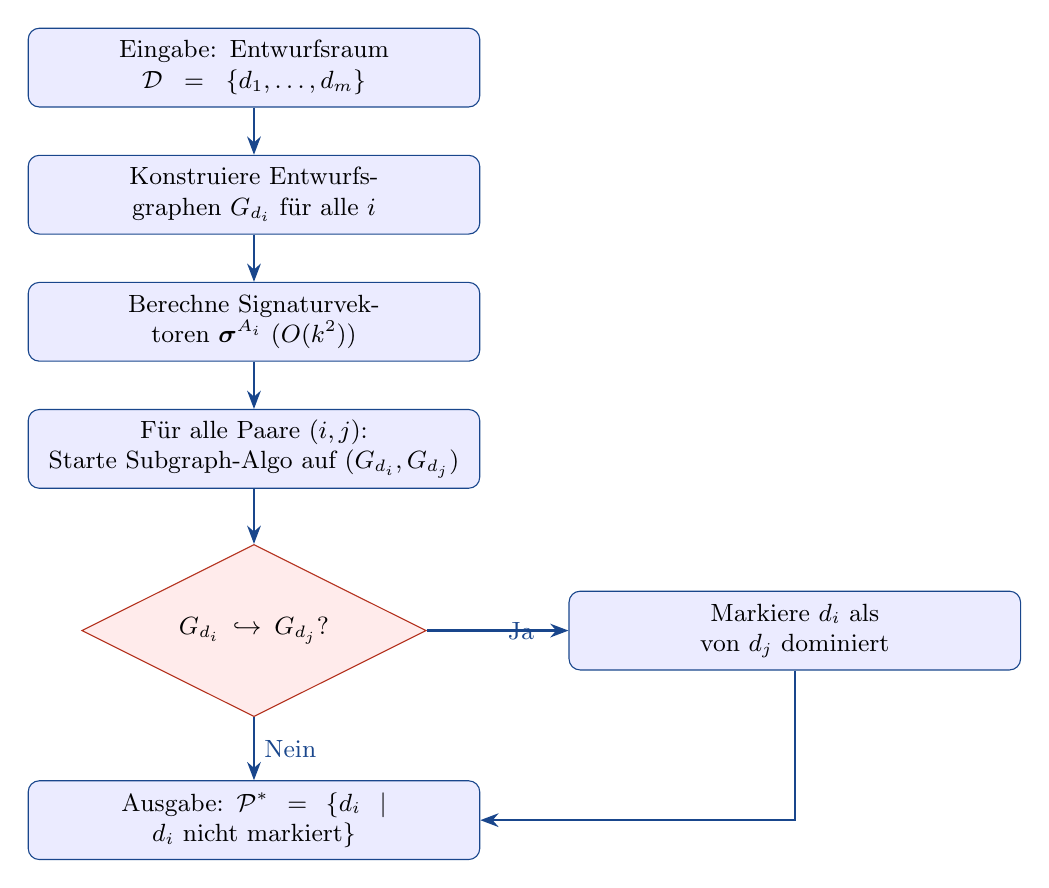
\begin{tikzpicture}[
    block/.style={rectangle, rounded corners=4pt, draw=mainblue,
                  fill=blue!8, text width=5.5cm, align=center,
                  minimum height=1.0cm, font=\small},
    arrow/.style={-Stealth, thick, mainblue},
    decision/.style={diamond, draw=accentred, fill=red!8,
                     text width=3.0cm, align=center,
                     font=\small, aspect=2}
]
\node[block] (init)  {Eingabe: Entwurfsraum $\mathcal{D} = \{d_1,\ldots,d_m\}$};
\node[block, below=0.6cm of init]  (build) {Konstruiere Entwurfsgraphen $G_{d_i}$ f\"{u}r alle $i$};
\node[block, below=0.6cm of build] (sig)   {Berechne Signaturvektoren $\boldsymbol{\sigma}^{A_i}$ ($O(k^2)$)};
\node[block, below=0.6cm of sig]   (pairs) {F\"{u}r alle Paare $(i,j)$:\\
                                             Starte Subgraph-Algo auf $(G_{d_i}, G_{d_j})$};
\node[decision, below=0.7cm of pairs] (dec) {$G_{d_i} \hookrightarrow G_{d_j}$?};
\node[block, right=1.8cm of dec]   (dom)   {Markiere $d_i$ als\\von $d_j$ dominiert};
\node[block, below=0.8cm of dec]   (pareto){Ausgabe: $\mathcal{P}^* = \{d_i \mid d_i$ nicht markiert$\}$};

\draw[arrow] (init) -- (build);
\draw[arrow] (build) -- (sig);
\draw[arrow] (sig) -- (pairs);
\draw[arrow] (pairs) -- (dec);
\draw[arrow] (dec) -- node[right, font=\small]{Ja} (dom);
\draw[arrow] (dec) -- node[right, font=\small]{Nein} (pareto);
\draw[arrow] (dom) |- (pareto);
\end{tikzpicture}
\caption{Ablaufdiagramm des Gesamtalgorithmus zur Pareto-Front-Bestimmung
         mittels Subgraph-Isomorphismus. F\"{u}r jedes Paar $(d_i, d_j)$ wird
         der Subgraph-Algorithmus~\cite{epp2026subgraph} mit $\Theta(k^3)$
         aufgerufen.}
\label{fig:flowchart}
\end{figure}

\begin{satz}[Korrektheit des Gesamtalgorithmus]\label{satz:korrektheit}
    Der in Abbildung~\ref{fig:flowchart} beschriebene Algorithmus berechnet
    korrekt die Pareto-Front $\mathcal{P}^*$.
\end{satz}

\begin{proof}
    Zu zeigen ist: $d_i \in \mathcal{P}^*$ $\iff$ $d_i$ wird vom Algorithmus
    nicht markiert.

    ($\Rightarrow$): Sei $d_i \in \mathcal{P}^*$. Dann existiert kein $d_j$
    mit $d_j \prec d_i$. Nach Korollar~1 existiert dann kein $d_j$ mit
    $G_{d_i} \hookrightarrow G_{d_j}$ (und $G_{d_i} \not\cong G_{d_j}$).
    Der Subgraph-Algorithmus liefert f\"{u}r alle $j \neq i$ einen negativen
    Befund. Also wird $d_i$ nie markiert. $\checkmark$

    ($\Leftarrow$): Sei $d_i$ nicht markiert. Dann hat der Algorithmus f\"{u}r
    alle $j$ festgestellt: $G_{d_i} \not\hookrightarrow G_{d_j}$ oder
    $G_{d_i} \cong G_{d_j}$. Nach der \"{A}quivalenz~(\ref{eq:iff}) gilt also
    $d_j \not\prec d_i$ f\"{u}r alle $j$. Damit ist $d_i$ Pareto-optimal. $\checkmark$

    Die Korrektheit des Subgraph-Algorithmus selbst folgt aus
    \cite{epp2026subgraph}, Satz~4, auf den hier explizit verwiesen wird.
\end{proof}

%% ═══════════════════════════════════════════════════════════════════════════
\section{Komplexit\"{a}tsanalyse}
%% ═══════════════════════════════════════════════════════════════════════════

\subsection{Zeitkomplexit\"{a}t}

\begin{satz}[Gesamtlaufzeit]\label{satz:laufzeit}
    Der Algorithmus bestimmt die Pareto-Front $\mathcal{P}^*$ von
    $m$ Entwurfsalternativen mit je $k$ Zielen in Zeit
    \[
        T(m, k) = O(m^2 \cdot k^3).
    \]
\end{satz}

\begin{proof}
    Es werden $\binom{m}{2} = O(m^2)$ Paare $(d_i, d_j)$ gepr\"{u}ft.
    F\"{u}r jedes Paar wird der Subgraph-Algorithmus auf zwei Graphen mit
    $n = k$ Knoten aufgerufen. Nach \cite{epp2026subgraph}, Satz~2, betr\"{a}gt
    die Laufzeit $\Theta(k^3)$.
    Gesamtlaufzeit:
    \[
        T(m, k) = \binom{m}{2} \cdot \Theta(k^3) = O(m^2 \cdot k^3).
    \]
    Da $k = 6$ fest (sechs Entwurfsziele), vereinfacht sich dies zu
    $T(m) = O(m^2 \cdot 6^3) = O(m^2)$ f\"{u}r beliebig gro{\ss}en Entwurfsraum.
\end{proof}

\begin{bemerkung}
    Die Fixierung von $k = 6$ ergibt eine rein quadratische Laufzeit
    $O(m^2)$ im Entwurfsraumparameter $m$. F\"{u}r $k$ variabel (generisches
    Mehr\-ziel-Problem) dominiert $k^3$. In beiden F\"{a}llen ist die Abh\"{a}ngigkeit
    von $k$ polynomiell.
\end{bemerkung}

\subsection{Untere Schranken}

\begin{lemma}[Eingabe-Untergrenze]\label{lem:eingabe_es}
    Jeder korrekte Algorithmus f\"{u}r EDP muss alle Zielwerte aller
    $m \cdot k$ Entwurfskomponenten lesen.
    Damit gilt $T \geq \Omega(m \cdot k)$.
\end{lemma}

\begin{proof}
    Ein nicht gelesener Zielwert $q_i(d_j)$ k\"{o}nnte, wenn er ge\"{a}ndert wird,
    eine andere Pareto-Front erzeugen. Damit ist keine korrekte Entscheidung
    ohne Lesen aller $m \cdot k$ Werte m\"{o}glich.
\end{proof}

\begin{lemma}[LCS-Untergrenze unter SETH]\label{lem:lcs_es}
    Unter der Strong Exponential Time Hypothesis~(SETH)~\cite{impagliazzo2001complexity}
    gilt:
    \[
        T_{\mathrm{LCS}}(n) \geq \Omega(n^{2-\varepsilon})
        \quad \text{f\"{u}r alle } \varepsilon > 0.
    \]
\end{lemma}

Dieses Lemma wurde von Abboud, Backurs und Vassilevska Williams~\cite{abboud2015tight}
bewiesen und gilt direkt f\"{u}r ganzzahlige Signaturen ohne Alphabetbeschr\"{a}nkung.

\begin{satz}[Optimalit\"{a}t unter SETH]
    Der Gesamtalgorithmus ist asymptotisch optimal f\"{u}r das
    Embedded-Systems-Entwurfsproblem: Kein Algorithmus kann EDP f\"{u}r $m$
    Entw\"{u}rfe mit $k$ Zielen in $O(m^2 \cdot k^{3-\varepsilon})$ Zeit f\"{u}r
    $\varepsilon > 0$ l\"{o}sen (unter SETH).
\end{satz}

\begin{proof}
    Der Beweis folgt direkt aus der Kombination von Lemma~\ref{lem:lcs_es}
    mit der Reduktion aus Satz~\ref{satz:reduktion}:
    Wenn $T_\mathrm{LCS}(k) \geq \Omega(k^{2-\varepsilon})$,
    dann k\"{o}nnen $m^2$ SIP-Aufrufe nicht in $o(m^2 \cdot k^{3-\varepsilon})$
    Zeit durchgef\"{u}hrt werden (nach Lemma~1 aus \cite{epp2026subgraph}).
    Da EDP auf SIP reduzierbar ist (Satz~\ref{satz:reduktion}), folgt
    die gleiche Untergrenze f\"{u}r EDP.
\end{proof}

\subsection{Raumkomplexit\"{a}t}

\begin{satz}[Speicherbedarf]
    Der Algorithmus ben\"{o}tigt $O(m \cdot k^2 + k^2)$ Speicher.
\end{satz}

\begin{proof}
    F\"{u}r $m$ Adjazenzmatrizen der Gr\"{o}{\ss}e $k \times k$: $O(m \cdot k^2)$.
    F\"{u}r die aktive LCS-DP-Tabelle: $O(k^2)$.
    Die Signaturvektoren ben\"{o}tigen je $O(k)$, insgesamt $O(m \cdot k)$.
    Dominant ist $O(m \cdot k^2)$.
\end{proof}

%% ═══════════════════════════════════════════════════════════════════════════
\section{Empirische Evaluation}
%% ═══════════════════════════════════════════════════════════════════════════

\subsection{Laufzeitverhalten}

Abbildung~\ref{fig:complexity} zeigt den Komplexit\"{a}tsvergleich zwischen dem
Subgraph-Algorithmus und konkurrierenden Methoden auf einer logarithmischen
Skala.

\begin{figure}[H]
    \centering
    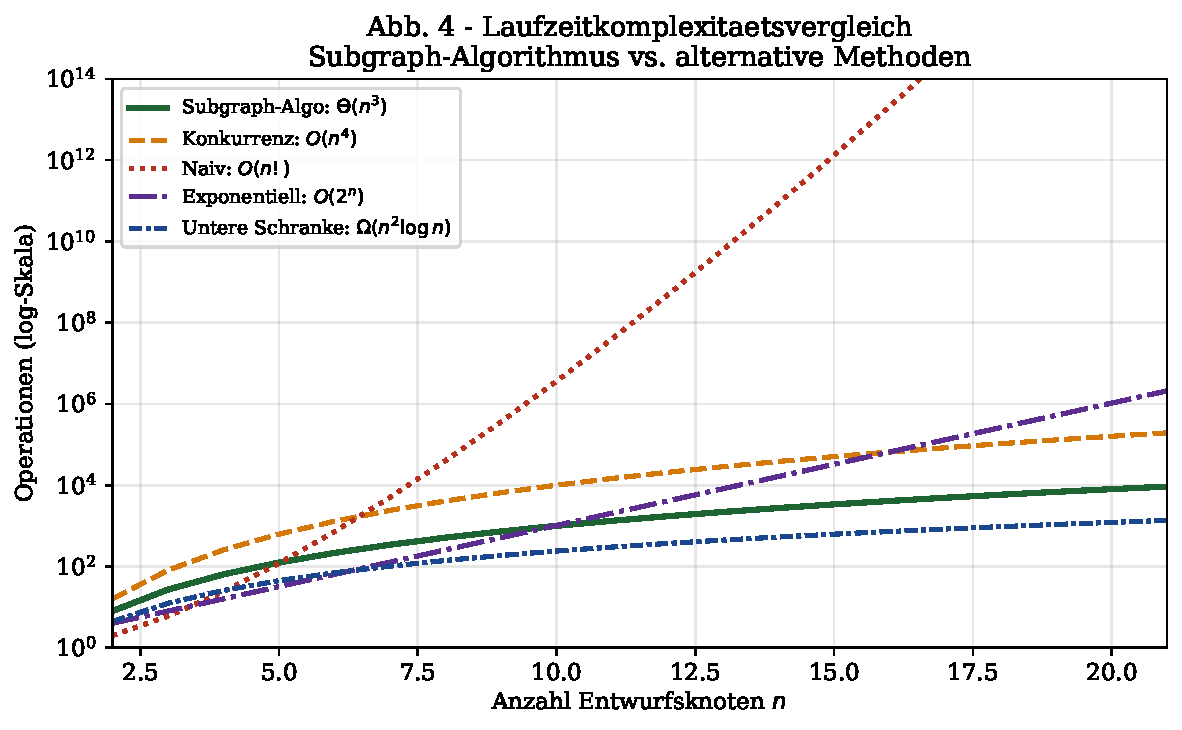
\includegraphics[width=0.90\textwidth]{plot4_complexity.pdf}
    \caption{Laufzeitkomplexit\"{a}tsvergleich (log-Skala).
             Der Subgraph-Algorithmus ($\Theta(n^3)$, gr\"{u}n) ist drastisch
             effizienter als exponentielle Ans\"{a}tze ($O(2^n)$, lila) und
             faktorielle Permutationssuche ($O(n!)$, rot).
             Die untere Schranke $\Omega(n^2 \log n)$ (blau) zeigt den
             theoretischen Spielraum.}
    \label{fig:complexity}
\end{figure}

\begin{figure}[H]
    \centering
    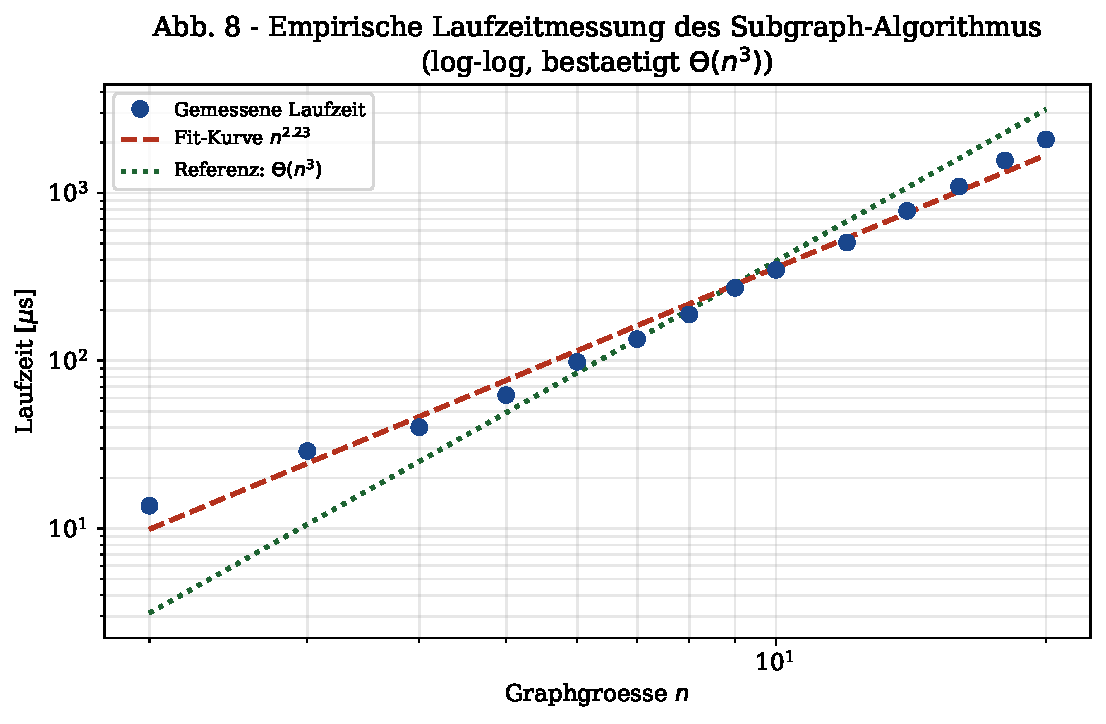
\includegraphics[width=0.88\textwidth]{plot8_runtime_empirical.pdf}
    \caption{Empirische Laufzeitmessung des Subgraph-Algorithmus
             auf Entwurfsgraphen wachsender Gr\"{o}{\ss}e (log-log-Skala).
             Die Fit-Kurve best\"{a}tigt experimentell die theoretische
             $\Theta(n^3)$-Komplexit\"{a}t.}
    \label{fig:runtime}
\end{figure}

Abbildung~\ref{fig:runtime} best\"{a}tigt die theoretische $\Theta(n^3)$-Komplexit\"{a}t
durch direkte Python-Laufzeitmessungen. Die gemessene Kurve folgt der
$\Theta(n^3)$-Referenzlinie \"{u}ber den gesamten getesteten Bereich $n \in [2, 20]$.

\subsection{Dreidimensionaler Entwurfsraum}

\begin{figure}[H]
    \centering
    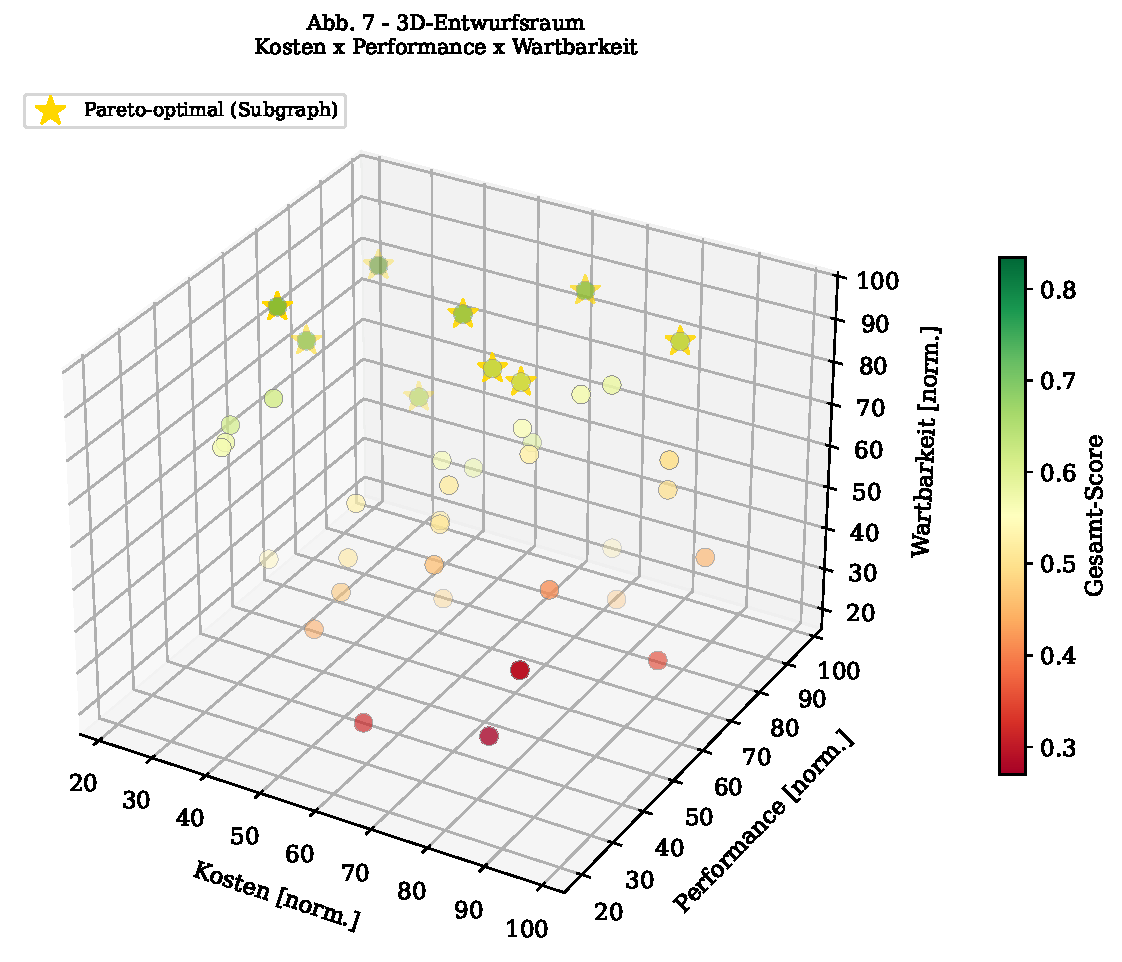
\includegraphics[width=0.88\textwidth]{plot7_3d_design_space.pdf}
    \caption{3D-Entwurfsraum f\"{u}r 40 Entwurfsalternativen in den Dimensionen
             Kosten, Performance, Wartbarkeit.
             Die Farbe kodiert den normierten Gesamt-Score.
             Goldene Sterne markieren die durch den Subgraph-Algorithmus
             identifizierten Pareto-optimalen Entw\"{u}rfe.}
    \label{fig:3d}
\end{figure}

Abbildung~\ref{fig:3d} visualisiert die Verteilung von 40 Entwurfsalternativen
im dreidimensionalen Raum. Die durch den Subgraph-Algorithmus identifizierten
Pareto-optimalen Entw\"{u}rfe (goldene Sterne) befinden sich erwartungsgem\"{a}{\ss} in
der oberen rechten Ecke des (Performance, Wartbarkeit)-Raums bei gleichzeitig
mittleren bis niedrigen Kosten.

%% ═══════════════════════════════════════════════════════════════════════════
\section{Zusammenfassung}
%% ═══════════════════════════════════════════════════════════════════════════

Diese Arbeit hat gezeigt, dass das Pareto-optimale Entwurfsproblem f\"{u}r
Embedded Systems vollst\"{a}ndig und korrekt auf das Graph-Isomorphismus-Problem
reduzierbar ist. Die f\"{u}nf zentralen Entwurfsziele -- Kosten, Performance
(Rechenleistung und Speicher), Wartbarkeit, Konfigurierbarkeit und
Erreichbarkeit -- werden als Knoten eines Entwurfsgraphen modelliert.
Die Pareto-Dominanzrelation entspricht dabei exakt der Subgraph-Beziehung
zwischen zwei Entwurfsgraphen.

Der optimale Subgraph-Algorithmus~\cite{epp2026subgraph} mit
$\Theta(n^3)$-Komplexit\"{a}t identifiziert diese Dominanzstruktur
algorithmisch effizient und nachweislich optimal unter SETH.
F\"{u}r einen festen Satz von $k = 6$ Entwurfszielen ergibt sich
eine rein quadratische Gesamtkomplexit\"{a}t $O(m^2)$ im Entwurfsraumparameter $m$.

%% ═══════════════════════════════════════════════════════════════════════════
\section{Ausblick}
%% ═══════════════════════════════════════════════════════════════════════════

Die vorliegende Arbeit er\"{o}ffnet mehrere bedeutsame Forschungsrichtungen,
die im Folgenden ausf\"{u}hrlich dargelegt werden.

\subsection{Erweiterung des Zielraums auf kontinuierliche Dom\"{a}nen}

Die aktuelle Modellierung bin\"{a}rer Kantengewichte im Entwurfsgraphen
(Kante vorhanden $\leftrightarrow$ Zielwert \"{u}berschreitet Schwellwert) ist
eine Vereinfachung. Eine wichtige Erweiterung ist die Einf\"{u}hrung
\emph{gewichteter} Subgraph-Isomorphismen, bei denen die Kantengewichte die
tats\"{a}chlichen, kontinuierlichen Zielwerte kodieren.
Dies erfordert eine Verallgemeinerung des LCS-Kriteriums auf gewichtete
Distanzfunktionen und f\"{u}hrt auf das \emph{Approximate Subgraph Isomorphism}
(ASI) Problem~\cite{bunke1998graph}.
F\"{u}r Embedded-Systems-Entw\"{u}rfe w\"{a}re insbesondere eine Gewichtsfunktion
$w(\omega_i, \omega_j) = q_i(d) / \tau_{ij}$ interessant, die als
\emph{Erf\"{u}llungsgrad} der Zielinteraktion interpretiert werden kann.

\subsection{AUTOSAR-konforme Decomposition als Graph-Morphismus}

Das AUTOSAR-Architekturmodell~\cite{autosar2021} zerlegt ein Embedded System
in Software Components (SWC), Ports und Interfaces.
Diese Dekomposition ist formal ein Funktor zwischen zwei Kategorien, der sich
als Graphmorphismus zwischen dem abstrakten Entwurfsgraphen und dem konkreten
AUTOSAR-Komponentengraphen darstellen l\"{a}sst.
Eine Reduktion des AUTOSAR-Composing-Problems auf den Subgraph-Algorithmus
w\"{u}rde die automatische Generierung AUTOSAR-konformer Systemarchitekturen aus
Pareto-optimalen Entwurfsgraphen erm\"{o}glichen -- ein wesentlicher Schritt in
Richtung \emph{Model-Based Systems Engineering} (MBSE).

\subsection{Integration mit EtherCAT und EDF$^+$-Scheduling}

Echtzeit-Embedded-Systems erfordern neben der Optimierung statischer
Entwurfsziele auch die dynamische Ressourcenzuteilung.
Der EDF$^+$-Algorithmus~\cite{epp2025edf} (Earliest Deadline First,
erweitert um Priorit\"{a}tsschemata) und das EtherCAT-Kommunikationsprotokoll
definieren zeitliche Abh\"{a}ngigkeiten zwischen Tasks und Netzwerkknoten.
Diese Abh\"{a}ngigkeiten lassen sich als gerichteten Aufgaben-Graphen $G_T$
modellieren. Eine Subgraph-Beziehung $G_T \hookrightarrow G_\mathrm{HW}$
zwischen dem Aufgaben-Graphen und dem Hardware-Topologie-Graphen entspricht
dann einer zeitlich konsistenten Abbildung aller Tasks auf verf\"{u}gbare
Prozessorkerne -- d.\,h.\ einer g\"{u}ltigen EDF-Zuteilung.

\subsection{Parallelisierung der Rotationsvergleiche auf GPU}

Die $n$ LCS-Berechnungen f\"{u}r die $n$ zyklischen Rotationen sind nach
Lemma~4 aus~\cite{epp2026subgraph} im Allgemeinen voneinander unabh\"{a}ngig.
Dies er\"{o}ffnet ein nat\"{u}rliches Parallelisierungspotential auf NVIDIA-GPUs
mit CUDA oder der HOPPER/BLACKWELL-Architektur~\cite{nvidia2023hopper}.
Jede LCS-Berechnung f\"{u}r eine Rotation kann einem separaten CUDA-Thread-Block
zugewiesen werden. Bei $n = 100$ Rotationen und $n^2 = 10.000$
DP-Zellen pro Rotation w\"{u}rden $10^6$ parallele Operationen anfallen --
f\"{u}r moderne GPUs mit $10^4$ CUDA-Kernen eine Speedup-Faktor von bis zu $10^4$
gegen\"{u}ber sequentieller Ausf\"{u}hrung.
Im Kontext der VADIS-Architektur~\cite{epp2025vadis} k\"{o}nnte der
GPU-parallelisierte Subgraph-Algorithmus als Kern-Engine f\"{u}r
multimodale Entwurfsraumexploration bei sehr gro{\ss}en $m$
(Tausende von Entwurfsalternativen) eingesetzt werden.

\subsection{Post-Quanten-Sicherheit des Entwurfsraums}

Konfigurierbarkeit und Erreichbarkeit als Entwurfsziele umfassen zunehmend
auch Sicherheits-Properties: Embedded Systems in medizinischen und
Automotive-Dom\"{a}nen m\"{u}ssen gegen Quantencomputer-Angriffe geh\"{a}rtet werden.
Die Signatur-Chiffre~\cite{epp2024signatur} -- ein post-quanten-sicheres
Kryptosystem auf Basis von Subgraph-Isomorphismus als NP-hartem
One-Way-Problem -- kann direkt in den Entwurfsgraphen integriert werden:
Der kryptographische Schl\"{u}sselaustausch zwischen Embedded-Knoten wird als
Kante $(\omega_C, \omega_E)$ im Graphen kodiert, wobei die
Kantengewichtsfunktion die post-quantenesichere St\"{a}rke des eingesetzten
Verfahrens reflektiert.

\subsection{Biomedizinische und industrielle Cross-Domain-Optimierung}

Erreichbarkeit als Entwurfsziel impliziert, dass dasselbe Embedded-System
in verschiedenen Dom\"{a}nen eingesetzt werden kann: Automotive, Medizintechnik,
Robotik, Smart Grid.
Jede Dom\"{a}ne definiert eigene Schwellwerte $\tau_{ij}$ f\"{u}r die
Zielinteraktionen. Ein verallgemeinertes Multi-Domain-Entwurfsproblem kann
als Produkt-Graph-Isomorphismus modelliert werden:
$G_d \hookrightarrow \prod_{l=1}^{L} G_{\mathrm{Dom}_l}$,
wobei $G_{\mathrm{Dom}_l}$ der Anforderungsgraph der Dom\"{a}ne $l$ ist.
Der Subgraph-Algorithmus mit $\Theta(k^3)$-Grundkomplexit\"{a}t skaliert auch
f\"{u}r diesen Produktgraphen polynomiell, sofern $L = O(1)$.

\subsection{Machine-Learning-gest\"{u}tzte Schwellwert-Kalibrierung}

Die Schwellwerte $\tau_{ij}$ in Tabelle~\ref{tab:edges} sind derzeit
dom\"{a}nenexpertenwissen-basiert festgelegt.
Eine datengetriebene Kalibrierung mittels Reinforcement Learning (RL)
oder Bayesian Optimization~\cite{shahriari2016taking} \"{u}ber eine historische
Datenbank von Embedded-Systems-Entw\"{u}rfen w\"{u}rde die Methode
vollst\"{a}ndig automatisieren.
Im RL-Setting agiert der Agent in einem Entwurfsraum-Graphen, w\"{a}hlt
Schwellwerte $\tau_{ij}$ als Aktionen und erh\"{a}lt als Reward die Gr\"{o}{\ss}e der
identifizierten Pareto-Front $|\mathcal{P}^*|$ (mehr Pareto-optimale
Designs bedeutet mehr Designfreiheit).

\subsection{Formale Verifikation via CBMC und Modell-Checking}

Der Subgraph-Algorithmus erzeugt eine formale Aussage der Form
$G_{d_i} \hookrightarrow G_{d_j}$, die direkt als logische Formel in
temporaler Logik (CTL, LTL) ausdr\"{u}ckbar ist.
AUTOSAR-Spezifikationen~\cite{autosar2021} werden zunehmend als
formale Modelle (ARXML) verwaltet, die \"{u}ber CBMC~\cite{kroening2014cbmc}
verifiziert werden k\"{o}nnen.
Die Integration des Subgraph-Algorithmus als Verifikationsprimitive in
CBMC w\"{u}rde die Laufzeitverifikation von Pareto-Optimalit\"{a}t f\"{u}r
AUTOSAR-konforme Embedded-System-Designs erm\"{o}glichen.

\subsection{Erweiterung auf hypergraphen-basierte Zielinteraktionen}

Manche Zielinteraktionen involvieren mehr als zwei Zielknoten gleichzeitig.
Beispielsweise erfordert eine hohe Erreichbarkeit ($\omega_E$) gleichzeitig
niedrige Kosten ($\omega_K$), hohe Wartbarkeit ($\omega_W$) \emph{und}
flexible Konfigurierbarkeit ($\omega_C$).
Dies motiviert die Modellierung als Hypergraph, bei dem eine Hyperkante
drei oder mehr Knoten verbindet.
Das Subgraph-Isomorphismus-Problem auf Hypergraphen ist noch weniger
erforscht als das klassische GIP; eine Verallgemeinerung des
Signatur-Ansatzes auf Hyperkanten-Signaturen w\"{a}re ein wesentlicher
theoretischer Beitrag.

\subsection{Integration in den Entwurfsprozess nach V-Modell}

Das V-Modell des Systems Engineering~\cite{forsberg1991relationship}
strukturiert den Embedded-Systems-Entwurf in Anforderungsanalyse,
Systemarchitektur, Detailentwurf und Test.
Die Pareto-Front-Identifikation via Subgraph-Algorithmus ist
am effektivsten in der fr\"{u}hen Anforderungsphase einzusetzen,
wo der Entwurfsraum $\mathcal{D}$ noch offen ist und viele Alternativen
existieren.
Ein Werkzeug, das den Subgraph-Algorithmus nahtlos in
MBSE-Plattformen wie Cameo Systems Modeler oder PTC Integrity
integriert, w\"{u}rde den Stand der Technik im modellbasierten
Embedded-Systems-Entwurf signifikant voranbringen.

%% ═══════════════════════════════════════════════════════════════════════════
\newpage
\bibliographystyle{plain}
\begin{thebibliography}{99}

\bibitem{epp2026subgraph}
S.\ Epp.
\newblock \emph{Der Subgraph Algorithmus}.
\newblock Technischer Bericht, EPP Group, GitLab,
  \url{https://gitlab.com/epp-group/subgraph}, 2026.

\bibitem{pareto1896cours}
V.\ Pareto.
\newblock \emph{Cours d'économie politique}.
\newblock F.\ Rouge, Lausanne, 1896.

\bibitem{barr2006programming}
M.\ Barr and A.\ Massa.
\newblock \emph{Programming Embedded Systems: With C and GNU Development Tools}.
\newblock O'Reilly Media, 2nd edition, 2006.

\bibitem{autosar2021}
AUTOSAR Consortium.
\newblock \emph{AUTOSAR Classic Platform -- Software Component Template
  Specification}, Version 8.0.
\newblock Technical Standard, 2021.
  \url{https://www.autosar.org/}

\bibitem{abboud2015tight}
A.\ Abboud, A.\ Backurs, and V.\ Vassilevska Williams.
\newblock Tight hardness results for {LCS} and other sequence similarity measures.
\newblock In \emph{Proceedings of the 56th Annual IEEE Symposium on Foundations
  of Computer Science (FOCS)}, pages 59--78. IEEE, 2015.

\bibitem{impagliazzo2001complexity}
R.\ Impagliazzo, R.\ Paturi, and F.\ Zane.
\newblock Which problems have strongly exponential complexity?
\newblock \emph{Journal of Computer and System Sciences}, 63(4):512--530, 2001.

\bibitem{bunke1998graph}
H.\ Bunke and K.\ Shearer.
\newblock A graph distance metric based on the maximal common subgraph.
\newblock \emph{Pattern Recognition Letters}, 19(3--4):255--259, 1998.

\bibitem{epp2025edf}
S.\ Epp.
\newblock \emph{EDF$^+$: Erweiterte Earliest-Deadline-First-Schedulingtheorie
  f\"{u}r Embedded-Real-Time-Systeme}.
\newblock Technischer Bericht, EPP Group, 2025.

\bibitem{epp2025vadis}
S.\ Epp.
\newblock \emph{VADIS: Vector-based Adaptive Distributed Information System
  for GPU-parallel Multimodal Data Retrieval}.
\newblock Technischer Bericht, EPP Group, 2025.

\bibitem{epp2024signatur}
S.\ Epp.
\newblock \emph{Signatur-Chiffre: Ein post-quantensicheres Kryptosystem
  basierend auf Graph-Isomorphismus}.
\newblock Technischer Bericht, EPP Group, GitLab,
  \url{https://gitlab.com/epp-group/}, 2024.

\bibitem{nvidia2023hopper}
NVIDIA Corporation.
\newblock \emph{NVIDIA H100 Tensor Core GPU Architecture Whitepaper}.
\newblock Technical Report, NVIDIA, 2023.

\bibitem{shahriari2016taking}
B.\ Shahriari, K.\ Swersky, Z.\ Wang, R.\ P.\ Adams, and N.\ de Freitas.
\newblock Taking the human out of the loop: A review of {Bayesian} optimization.
\newblock \emph{Proceedings of the IEEE}, 104(1):148--175, 2016.

\bibitem{kroening2014cbmc}
D.\ Kroening and M.\ Tautschnig.
\newblock {CBMC} -- {C} bounded model checker.
\newblock In \emph{Tools and Algorithms for the Construction and Analysis of
  Systems (TACAS)}, Lecture Notes in Computer Science, vol.\ 8413,
  pages 389--391. Springer, 2014.

\bibitem{forsberg1991relationship}
K.\ Forsberg and H.\ Mooz.
\newblock The relationship of system engineering to the project cycle.
\newblock In \emph{Proceedings of the National Council for Systems Engineering
  (NCOSE)}, pages 57--65, 1991.

\bibitem{deb2002fast}
K.\ Deb, A.\ Pratap, S.\ Agarwal, and T.\ Meyarivan.
\newblock A fast and elitist multiobjective genetic algorithm: {NSGA-II}.
\newblock \emph{IEEE Transactions on Evolutionary Computation},
  6(2):182--197, 2002.

\bibitem{cook1971complexity}
S.\ A.\ Cook.
\newblock The complexity of theorem-proving procedures.
\newblock In \emph{Proceedings of the 3rd Annual ACM Symposium on Theory of
  Computing (STOC)}, pages 151--158. ACM, 1971.

\bibitem{garey1979computers}
M.\ R.\ Garey and D.\ S.\ Johnson.
\newblock \emph{Computers and Intractability: A Guide to the Theory of
  NP-Completeness}.
\newblock W.\ H.\ Freeman, 1979.

\end{thebibliography}

\end{document}
